\subsection{Symptomer}
KOL udvikles over mange år, dog vil patienten ikke bemærke sygdommen førend lungefunktionen er markant nedsat. Dette betyder, at KOL og dens symptomer som regel først kommer til udtryk efter 50 års-alderen\cite{Lange2015}. Dette kan betyde, at patienter først opsøger en læge, når deres lungefunktion er halveret \cite{dsam2016}.

Symptomer på KOL er åndenød og hoste ved fysisk aktivitet, der kan være med ekspektoration, som hos de fleste KOL patienter er klart eller hvidt.\cite{Basisbogen2016} Derudover er der en tendens til hyppig eksacerbationer, hvilket er tilfælde, hvor KOL-patienters tilstand forværres akut og kræver behandling. 
Symptomerne herunder opleves som øget åndenød, hoste samt grønt eller gulligt ekspektoration og øget purulens. Denne tilstand skyldes ofte infektioner med bakterier, hvilket udgør ca. 50 \% af tilfældene. Derudover kan virale infektioner samt luftforurening resultere i, at KOL-patienter oplever eksacerbationer.\cite{Basisbogen2016, dsam2016} 

Der er en række komorbiditeter, som hyppigt ses hos KOL-patienter, som desuden kan have en negativ påvirkning på patienternes livskvalitet og prognose. Ved årskontroller bør patienten tjekkes for de hyppigste komormiditeter; kardiovaskulære sygdomme, type-2 diabetes, osteoporose, lungecancer, muskelsvækkelse samt angst og depression.
Nogle af komorbiditeterne kan skyldes, at åndenød har medført et nedsat fysisk aktivitetsniveau og dermed svage perifere muskler samt vægttab. Desuden har rygning og generelt dårlig livsstil ligeledes betydning for udviklingen af disse komorbiditeter. \cite{dsam2016, McCarthy2015}
Psykiske komorbiditeter, ofte i form af depression og angst, har en øget forekomst hos patienter med en FEV1 værdi på under 50 \% af den forventede værdi. Desuden kan angst og depression udløses ved diagnosen af KOL. Den øgede risiko for psykiske lidelser skyldes, at KOL kan medføre social isolation og tab af sociale relationer, skyldfølelse, usikkerhed med hensyn til fremtiden. \cite{dsam2016}


\subsection{Diagnose}
Ved mistanke om KOL undersøges lungefunktionen ved spirometriundersøgelser, hvor FEV1 og FVC måles. Patienten foretager en maksimal inspiration, hvorefter FEV1 er den volumen, som udåndes i det første sekund af en forceret eksspiration. Denne værdi giver information om hastigheden, hvormed lungerne tømmes. FVC er en indikator for lungevolumen. Af \autoref{fig:FEV} ses spirometrimålinger for henholdsvis patient med normal, obstruktiv og restriktiv nedsat lungefunktion samt en kombination af disse.\cite{Basisbogen2016, Sundhed2013}

\begin{figure} [H]
\centering
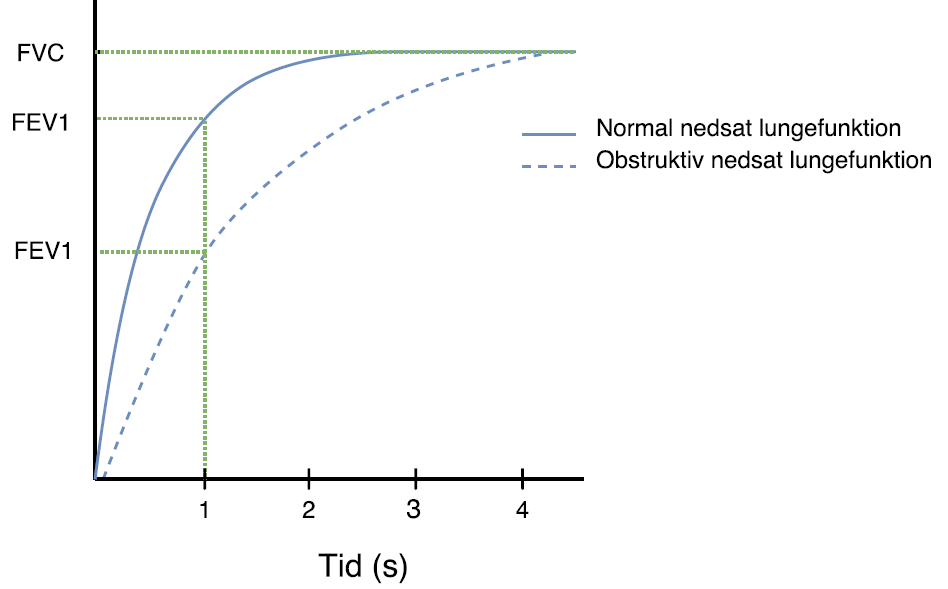
\includegraphics[width=0.5\textwidth]{figures/FEV}
\caption{Spirometrimålinger for patient med normal, obstruktivt og restriktiv nedsat lungefunktion samt en patient med kombineret obstruktivt og restriktivt nedsat lungefunktion.}
\label{fig:FEV}
\end{figure} 

\noindent
Det fremgår af \autoref{fig:FEV}, at der fald i FEV1 ved nedsat lungefunktion. Dertil ses det ligeledes, at patienter med nedsat lungefunktion har fald i lungevolumen (FVC). Som tidligere nævnt vil obstruktivt nedsat lungefunktion ses ved en FEV1/FVC-ratio på under 70 \% af den forventede værdi. 
Der udføres desuden en reversibilitetstest for at sikre, at patienten ikke lider af astma. Her gives patienten broncodilatorer, som hos astmapatienter vil forbedre spirometrimålingen, mens lungefunktionen for KOL-patienter forbliver uændret.\cite{Basisbogen2016, Sundhed2013} 
For at undersøge KOL og komobiditeter, som er forbundet med KOL undersøges foruden lungefunktionsundersøgelser BMI, røntgen af thorax, EKG-målinger og blodprøver \cite{Sundhed2013}. 
%Med tiden kan symptomerne på KOL forværres, og der skal mindre fysisk aktivitet til for at udløse åndenød. \cite{Basisbogen2016}